\documentclass[11pt]{article}

% Reference: https://www.overleaf.com/learn/latex/TikZ_package
% Reference: https://tikz.dev/library-shapes

\usepackage[a4paper, total={6in, 8in}]{geometry}
% tikz package is required to use TikZ in LaTeX document.
\usepackage{tikz}

% shapes.geometric is a TikZ library defining basic geometric objects.
\usetikzlibrary{shapes.geometric}
% We can define a custom TikZ style using \tikzstyle command.
\tikzstyle{cse300} = [draw, rectangle, draw=green, fill=green!50, thick, text width=3cm, text centered]

\title{Graphical Drawing in \LaTeX with Ti\textit{k}Z}
\author{Ajmain Yasar Ahmed Sahil}
\date{\today}

\begin{document}
    \maketitle
    
    \section*{Drawing Point, Lines \& Curves}
    
    \begin{tikzpicture}
        \draw[gray, thick, <->] (-4, 0) -- (4, 0);  % Straight Line
        \draw[gray, thick, <->] (0, -4) -- (0, 4);  % Straight Line
        \fill[black] (0, 0) circle (2pt);  % Point
        \draw[black, thick, -] (-3, 3) .. controls (-1, 1) and (1, 1) .. (3, 3);  % Bézier Curve
        \draw[black, thick, ->] (-3, -3) .. controls (0, -1) .. (3, -3);  % Bézier Curve
    \end{tikzpicture}
    
    \section*{Drawing Geometric Shapes}
    
    \begin{center}
        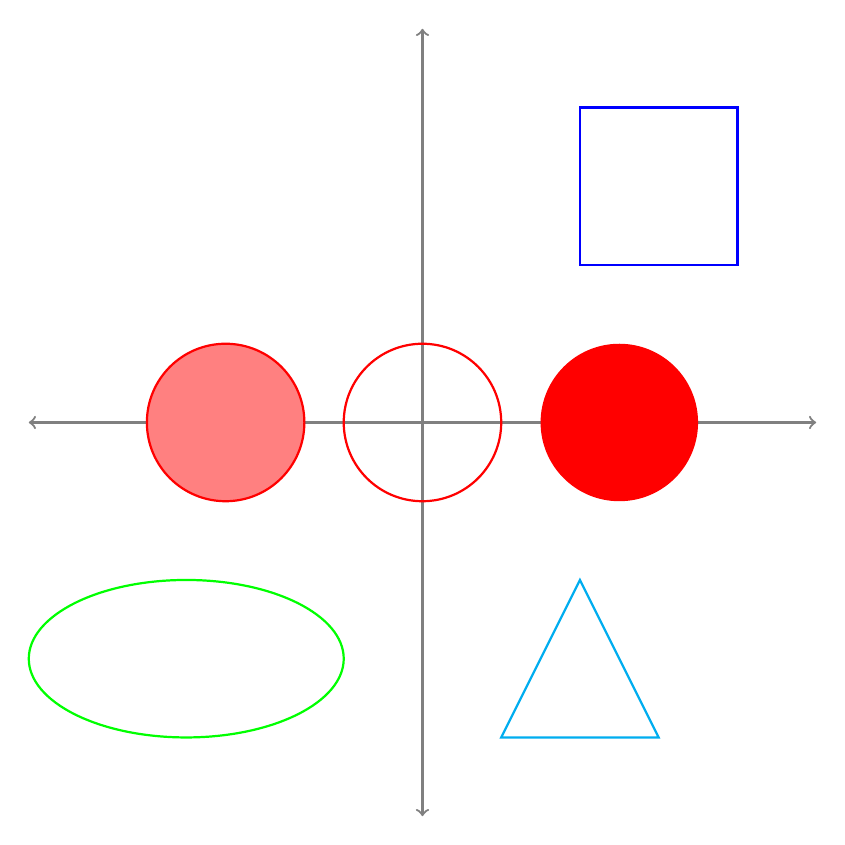
\begin{tikzpicture}
            \draw[gray, thick, <->] (-5, 0) -- (5, 0);
            \draw[gray, thick, <->] (0, -5) -- (0, 5);
            \draw[red, thick] (0, 0) circle (1);
            \fill[red] (2.5, 0) circle (1);
            \filldraw[draw=red, fill=red!50, thick] (-2.5, 0) circle (1);
            \draw[blue, thick] (2, 2) rectangle (4, 4);
            \draw[green, thick] (-3, -3) ellipse (2 and 1);
            \draw[cyan, thick] (1, -4) -- (3, -4) -- (2, -2) -- cycle;
        \end{tikzpicture}
    \end{center}
    
    \section*{Drawing Diagram}

    \begin{center}
        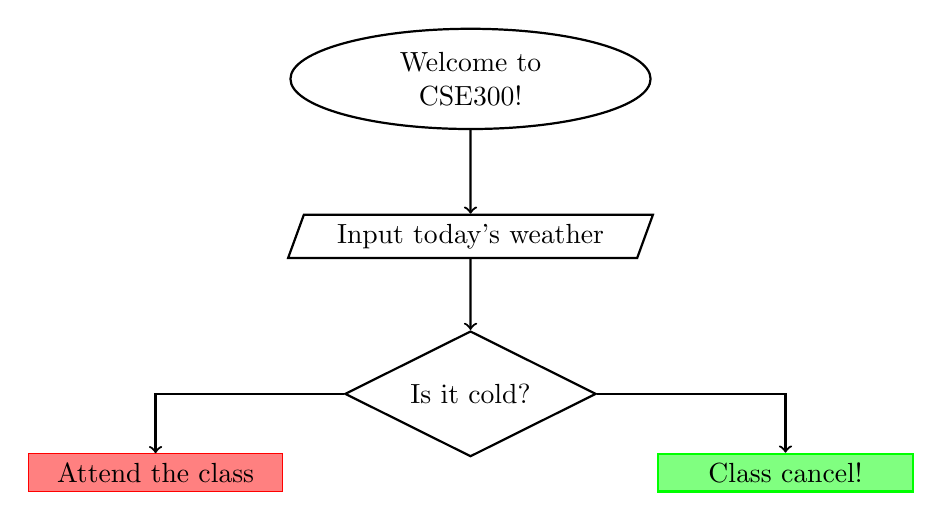
\begin{tikzpicture}
            % Defining nodes
            \node[draw, ellipse, black, thick, text width=3cm, text centered] (Begin) {Welcome to CSE300!};
            \node[draw, trapezium, black, thick, trapezium left angle=70, trapezium right angle=110, text width=4cm, text centered, below of=Begin, yshift=-1cm] (IO) {Input today's weather};
            \node[draw, diamond, black, thick, aspect=2, text width=2cm, text centered, below of=IO, yshift=-1cm] (Decision) {Is it cold?};
            \node[draw, rectangle, draw=red, fill=red!50, text width=3cm, text centered, left of=Decision, xshift=-3cm, yshift=-1cm] (Continue) {Attend the class};
            \node[cse300, right of=Decision, xshift=3cm, yshift=-1cm] (Cancel) {Class cancel!};
            
            % Drawing diagram
            \draw[black, thick, ->] (Begin.south) -- (IO.north);
            \draw[black, thick, ->] (IO.south) -- (Decision.north);
            \draw[black, thick, ->] (Decision.east) -| (Cancel.north);
            \draw[black, thick, ->] (Decision.west) -| (Continue.north);
        \end{tikzpicture}
    \end{center}
\end{document}